\documentclass{beamer}

\usepackage[T1]{fontenc}      % Para permitir correta hifenização/acentos
\usepackage[utf8]{inputenc}   % Arquivo LaTeX em UTF-8
\usepackage[portuguese]{babel} % Adapta formatação e termos para PT

\usetheme{Madrid}  % Pode escolher outro tema, se desejar

\title{Coisa é o Cálculo Paralelo e o High Performance Computing (HPC)\\
\textcolor{red}{\href{https://github.com/leodecarlo/TechWeb25}{https://github.com/leodecarlo/TechWeb25}}} 

\author{Leonardo De Carlo
(\textcolor{blue}{For a complete Tutorial: \emph{ \href{https://hpc.llnl.gov/documentation/tutorials/introduction-parallel-computing-tutorial}{https://hpc.llnl.gov/documentation/tutorials/introduction-parallel-computing-tutorial}}})}

\institute{CopeLab: AI and Complexity, Universidade Lusófona}

\date{\today}

	


\setbeamertemplate{footline}{} % Remove o rodapé completamente

\begin{document}
	
	%-------------------------------------------
	% Slide 1
	%-------------------------------------------
	\begin{frame}
		\titlepage
	\end{frame}
	
	%-------------------------------------------
	% Slide 2
	%-------------------------------------------
	\begin{frame}{Cálculo de \(\pi\) (Método de Monte Carlo)}
		
		\begin{columns}[T]
			% Coluna 1 (texto)
			\scriptsize
			\column{0.6\textwidth}
			\begin{itemize}
				\item Inscreva um círculo de raio \(r\) (área \(\pi r^2\)) dentro de um quadrado de lado \(2r\) (área \(4r^2\)).
				\item A razão entre a área do círculo e a do quadrado é: 
				\[
				\frac{\pi r^2}{4r^2} = \frac{\pi}{4};
				\]
				\item Gerando aleatoriamente \(N\) pontos dentro do quadrado, aproximadamente:  
				\[
				N \times \frac{\pi}{4};
				\]
				desses pontos (\(M\)) devem cair dentro do círculo.
				\item Assim, \(\pi\) pode ser aproximado por $N \times \frac{\pi}{4} = M$, então
				\[
				 \pi = 4 \times \frac{M}{N};
				\]
				\item Quanto maior o número de pontos gerados, melhor a aproximação.
			\end{itemize}
			
			% Coluna 2 (figura)
			\column{0.4\textwidth}
			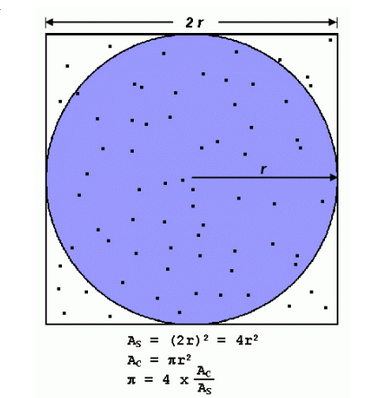
\includegraphics[scale=0.4]{circfig.png}
		\end{columns}
	\end{frame}
	
	%-------------------------------------------
	% Slide 3
	%-------------------------------------------
	\begin{frame}[fragile]{Pseudocódigo Serial}
		
		\begin{columns}[T]
			% Coluna 1 (código)
			\column{0.6\textwidth}
			\footnotesize
			\textbf{Pseudocódigo Serial:}
			\begin{verbatim}
				npoints = 10000
				circle_count = 0
				
				do j = 1,npoints
				generate 2 random numbers between 0 and 1
				xcoordinate = random1
				ycoordinate = random2
				if (xcoordinate, ycoordinate) inside circle
				circle_count = circle_count + 1
				end do
				
				PI = 4.0*circle_count/npoints
			\end{verbatim}
			
			% Coluna 2 (figura)
			\column{0.4\textwidth}
			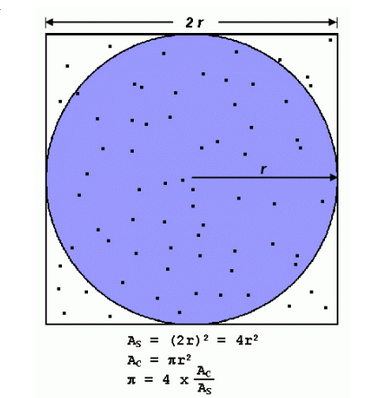
\includegraphics[scale=0.4]{circfig.png}
		\end{columns}
	\end{frame}
	
	%-------------------------------------------
	% Slide 4
	%-------------------------------------------
	\begin{frame}{Paralelização do Algoritmo}
		
		\begin{columns}[T]
			\column{0.6\textwidth}
			\footnotesize
			\textbf{Extensão para Paralelismo:}
			\begin{itemize}
				\item A contagem de $N$  pontos  é dividida entre os $n$ \textit{workers}(unidades computacionais), cada um processando uma parte da tarefa: $N/n$ pontos .
				\item Cada \textit{worker} calcula quantos pontos caem no círculo dentro do seu subconjunto.
				\item O \textit{master} recebe os resultados de todos os \textit{workers} e computa \(\pi\).
			\end{itemize}
			
			\textbf{Observações:}
			\begin{itemize}
				\item O cálculo de cada \textit{worker} é independente, ou seja, não precisa saber o que acontece com os outros. Em geral, isso não ocorre, pois muitas computações exigem comunicação entre \textit{workers}.
				\item O cálculo no passo de tempo \(n\) não depende dos passos anteriores. Isso é essencial para que a paralelização seja possível.
			\end{itemize}
			
			% Coluna 2 (figura)
			\column{0.4\textwidth}
			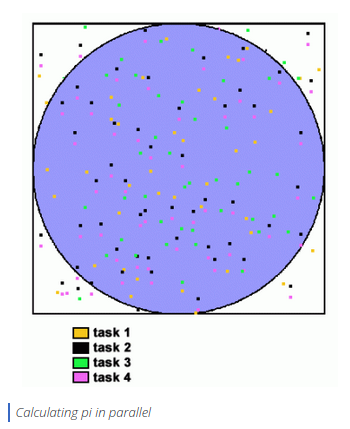
\includegraphics[scale=0.4]{par_circfig.png}
		\end{columns}
	\end{frame}
	
	%-------------------------------------------
	% Slide 5
	%-------------------------------------------
	\begin{frame}[fragile]{Pseudocódigo Paralelo (Visão Geral)}
		
		\begin{columns}[T]
			% Coluna 1 (código)
			\column{0.6\textwidth}
			\scriptsize
			\textbf{Pseudocódigo Paralelo:}
			\begin{verbatim}
				npoints = 10000
				circle_count = 0
				p = number_of_tasks
				num = npoints / p
				
				find out if I am MASTER or WORKER
				
				do j = 1, num
				generate random x, y in [0,1]
				if inside_circle(x,y)
				circle_count = circle_count + 1
				end do
				
				if I am MASTER
				receive circle_counts from WORKERS
				compute PI = 4.0*(total_circle_count)/npoints
				else
				send circle_count to MASTER
				end if
			\end{verbatim}
			
			% Coluna 2 (figura)
			\column{0.4\textwidth}
			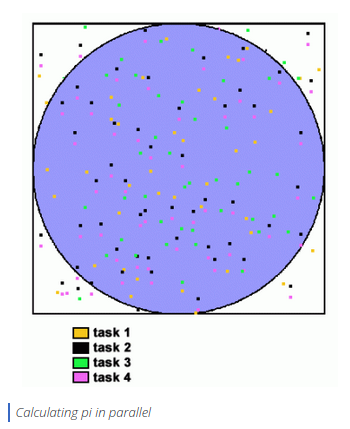
\includegraphics[scale=0.4]{par_circfig.png}
		\end{columns}
	\end{frame}
	
	%-------------------------------------------
	% Slide 6
	%-------------------------------------------
	\begin{frame}{Paralelização em Algoritmos Dependentes do Tempo}
		
		Muitas vezes, um algoritmo dependente da passos anteriores pode ser "\emph{paralelizado}".
		
		\vspace{0.2cm}
		 Sequência de Fibonacci (0,1,1,2,3,5,8,13,21,...),  usando a fórmula:
		
		\[
		F(n) = F(n-1) + F(n-2)
		\]
		
		O cálculo do valor \(F(n)\) depende dos valores de \(F(n-1)\) e \(F(n-2)\), que devem ser computados primeiro. Um algoritmo paralelo para resolver esse problema é usar a \textbf{fórmula de Binet}:
		
		\[
		F_n = \frac{\varphi^n - (-\varphi)^{-n}}{\sqrt{5}} = \frac{\varphi^n - (-\varphi)^{-n}}{2\varphi - 1},\,\,
		\varphi = \frac{1 + \sqrt{5}}{2} \approx 1.61803 39887\ldots
		\]
		
	\end{frame}
	
	\begin{frame}{High Performance Computing(HPC)}
		
		\scriptsize
		O cálculo paralelo está vivendo um momento de destaque com as últimas gerações de Graphic Processing Units (GPUs): uma capacidade de cálculo surpreendente no momento em que a Lei de Moore está chegando ao fim.
		
		\vspace{0.3cm}
		
		\begin{columns}[T] 
			% Coluna 1 (imagem)
			\column{0.5\textwidth}
			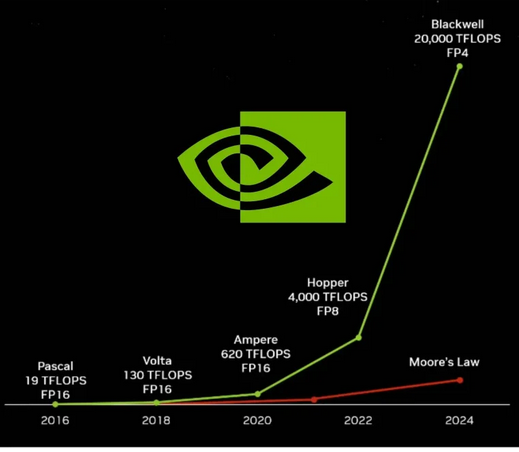
\includegraphics[scale=0.2]{Nvidia.png}
			
			% Coluna 2 (imagem)
			\column{0.5\textwidth}
			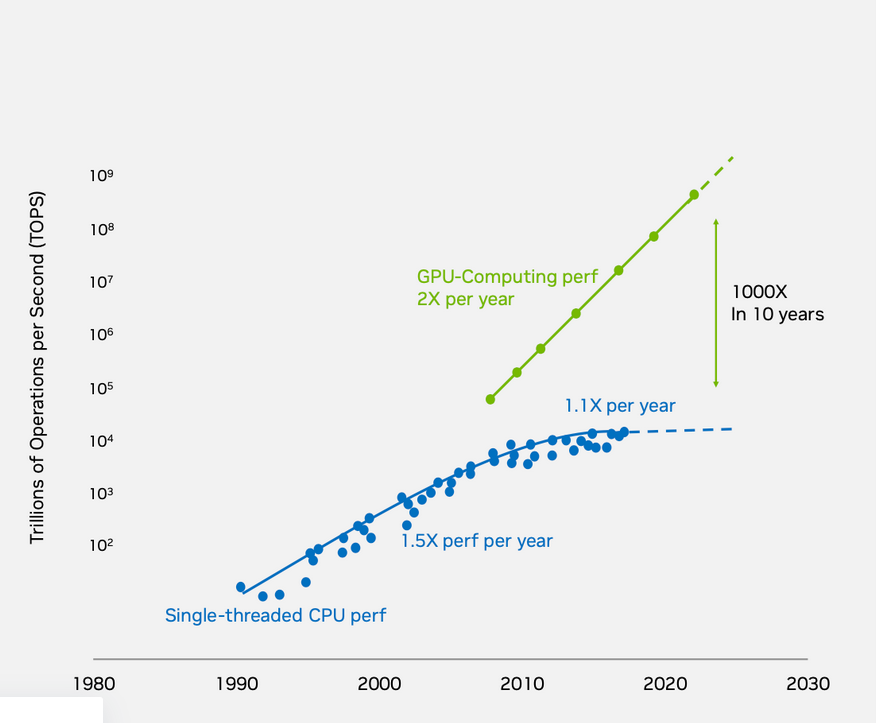
\includegraphics[scale=0.14]{Moore_vs_GPU.png}
		\end{columns}
		
		\vspace{0.3cm}
		
		Suceso graças a  conjunta  chegada de performante  I/O  datastorage:  massivo investimento da União Europeia (UE) em centros de HPC, \textcolor{blue}{\emph{\href{https://eurohpc-ju.europa.eu/index_en}{EuroHPC}}}
		(Resta provar que não estamos so enriquecendo os americanos: devido ao intenso I/O das GPUs, as vantagens dos clusters de GPUs(respeito CPUs) precisam ser demonstradas na maioria das situações (e.g. em sssimulações físicas)).
		
		\vspace{0.3cm}
		Essa nova tecnologia é a base para a explosão da popularização da inteligência artificial (AI). Outra aplicação de destaque é o uso de gêmeos digitais e simulações para a indústria.
		

	\end{frame}
	
\end{document}
